\section{Overview}\label{overview}

MicroTCA (uTCA) is Sinara's preferred form-factor for hardware with
high-speed data converters requiring deterministic phase control, such
as the \href{Sayma}{\emph{Sayma}} 2.4 GSPS smart arbitrary waveform
generator (SAWG).

uTCA is a modular, open standard originally developed by the
telecommunications industry. It allows a single rack master -- the Micro
TCA Carrier Hub (MCH) -- to control multiple slave boards, known as
Advanced Mezzanine Cards (AMCs) via a high-speed digital backplane. uTCA
chassis and backplanes are available commercially of the shelf (COTS).

We make use of the most recent extension to the uTCA standard, uTCA.4.
Originating in the high-energy and particle physics (HEPP) community,
uTCA.4 introduces rear-transition modules (RTMs) along with a second
backplane for low-noise RF signals (RFBP). Each RTM connects to an AMC
(one RTM per AMC). Typically, the AMCs hold FPGAs and other high-speed
digital hardware, communicating with the MCH via gigabit serial links
over the AMC backplane. The RTMs hold data converters and other
low-noise analog components, controlled by the corresponding AMC. The
RFBP provides low-noise clocks and local oscillators (LOs). The RTMs and
RFBP are screened from the AMCs to minimise interference from the
high-speed digital logic.

\begin{figure}[htbp!]
\centering
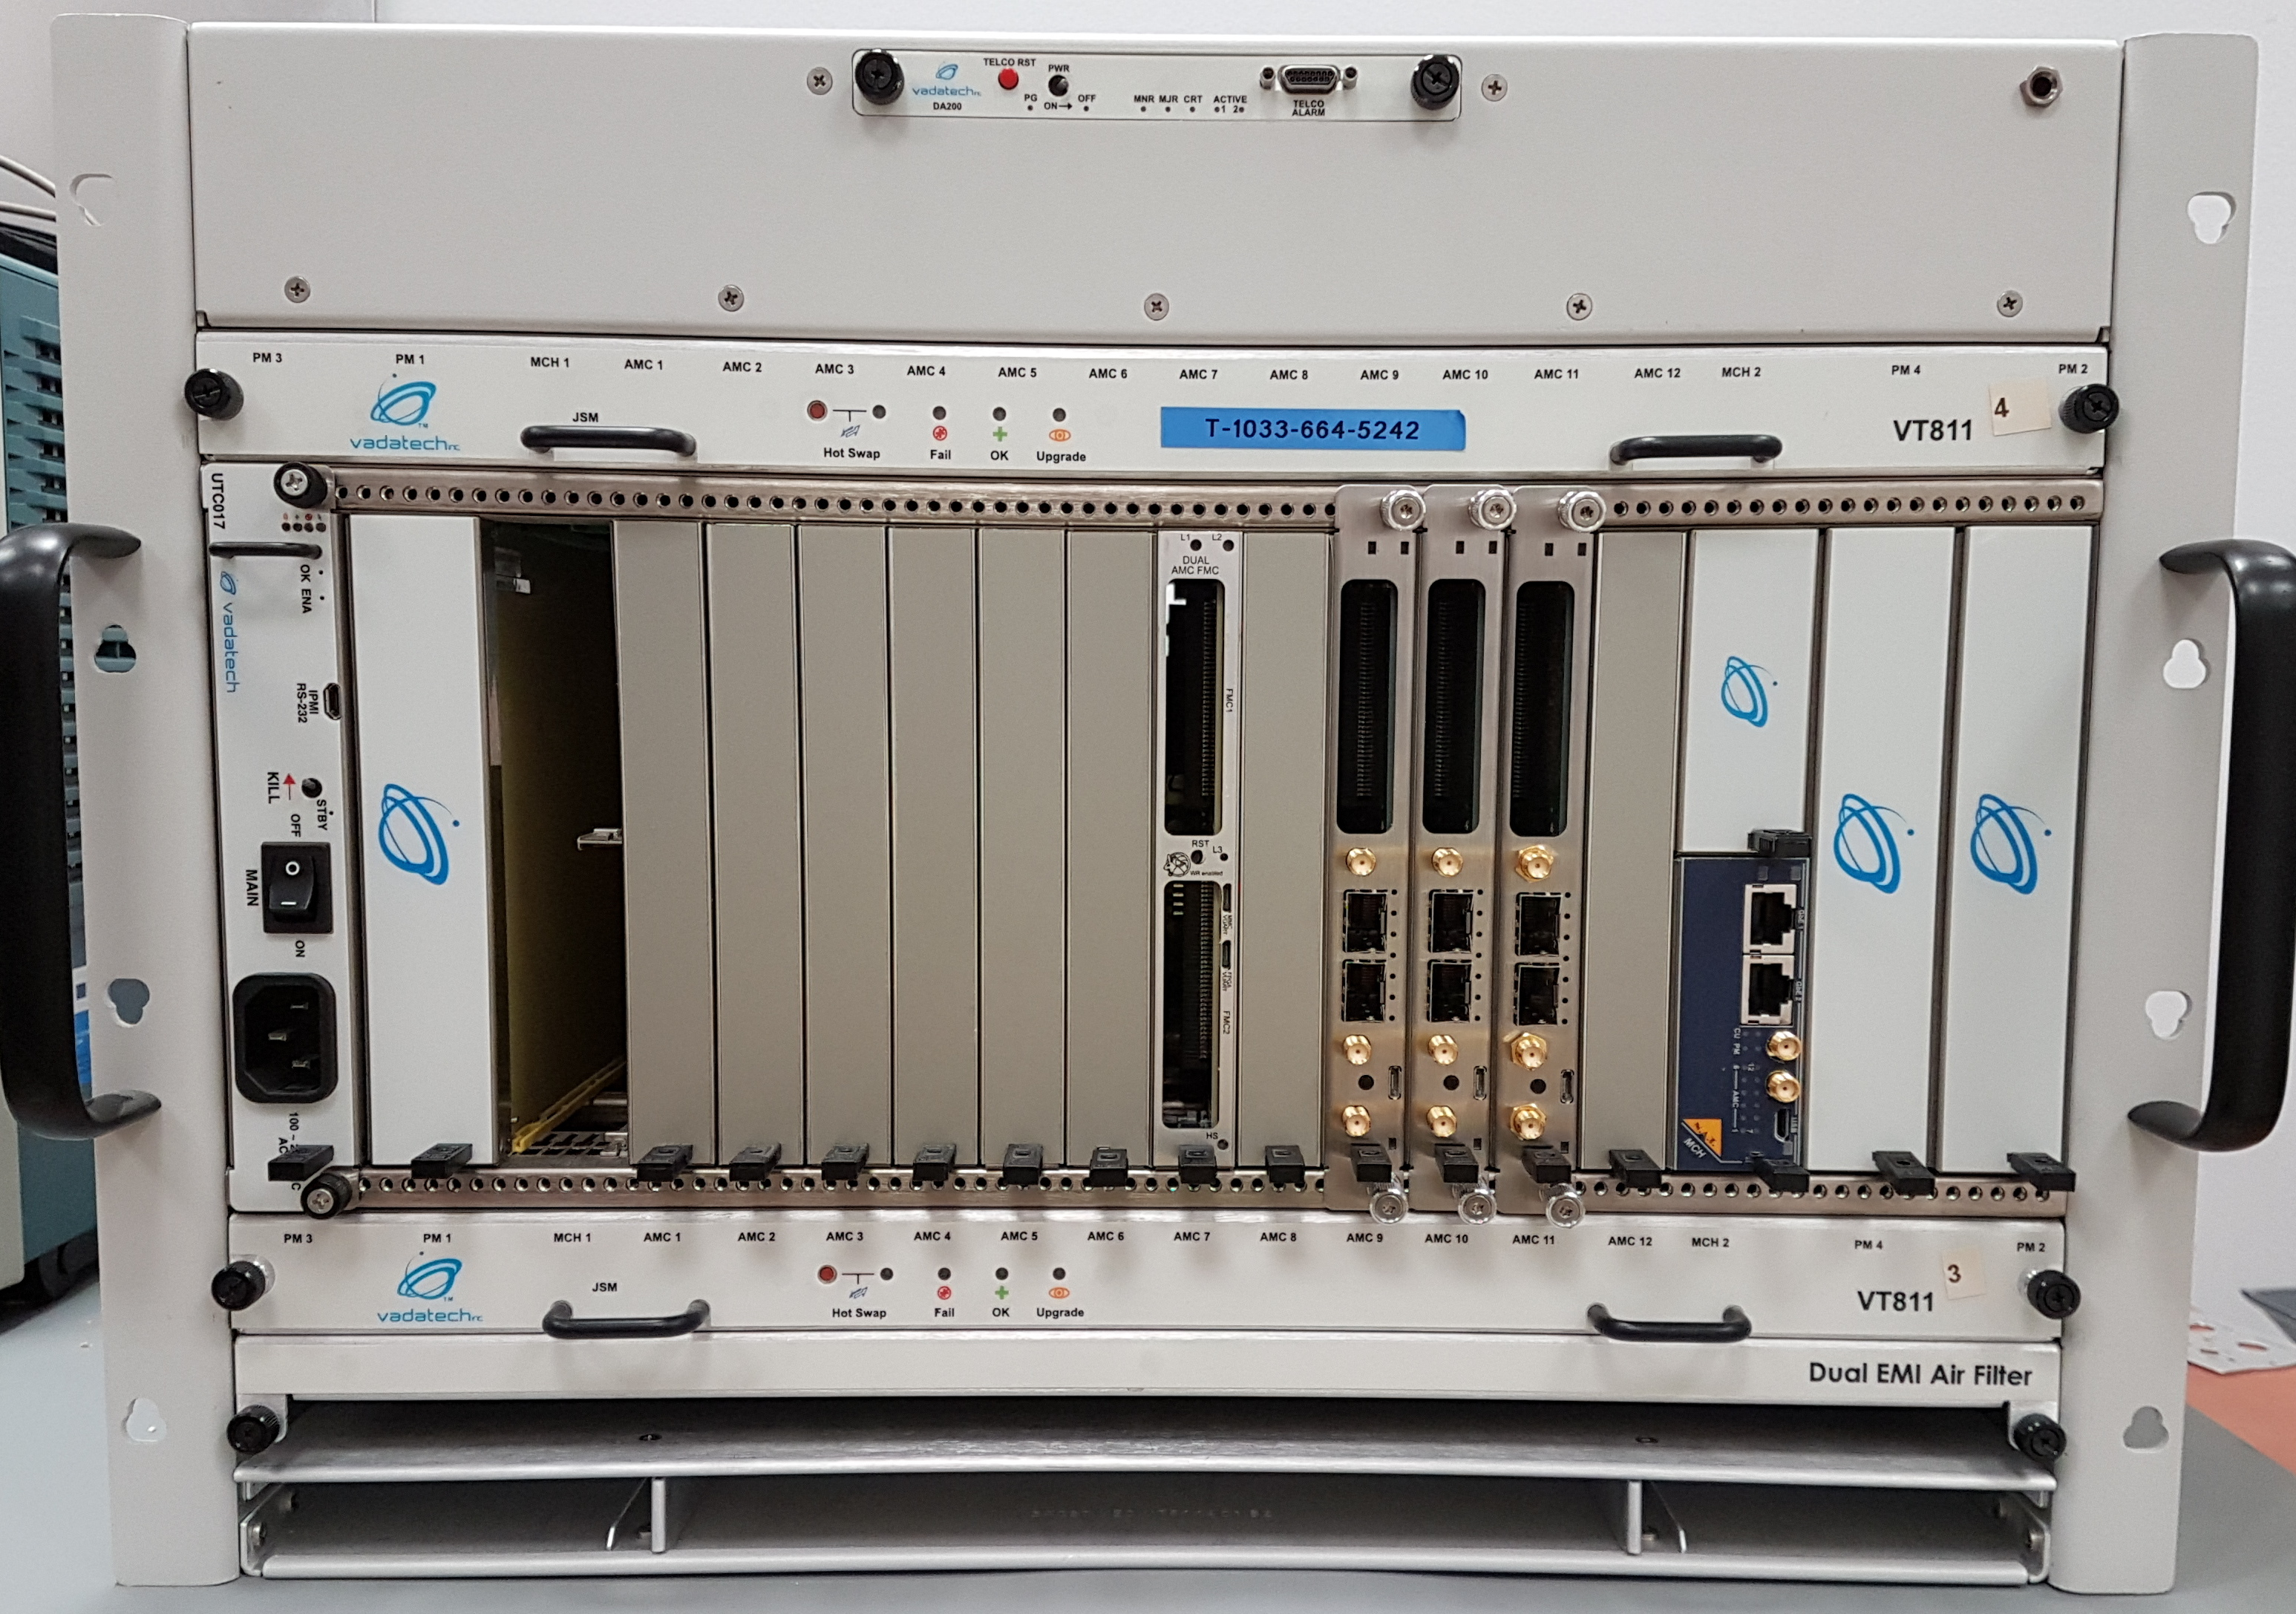
\includegraphics[width=15cm]{img/MTCA_Front.jpg}
\caption{Micro TCA chassis with 3 Sayma AMC modules inserted}
\end{figure}

(above) Micro TCA chassis with 3 Sayma AMC modules inserted.

Micro TCA chassis with 4 RTM modules inserted. One of them with 4
BaseMod AFE mezzanines installed.

\begin{figure}[htbp!]
\centering
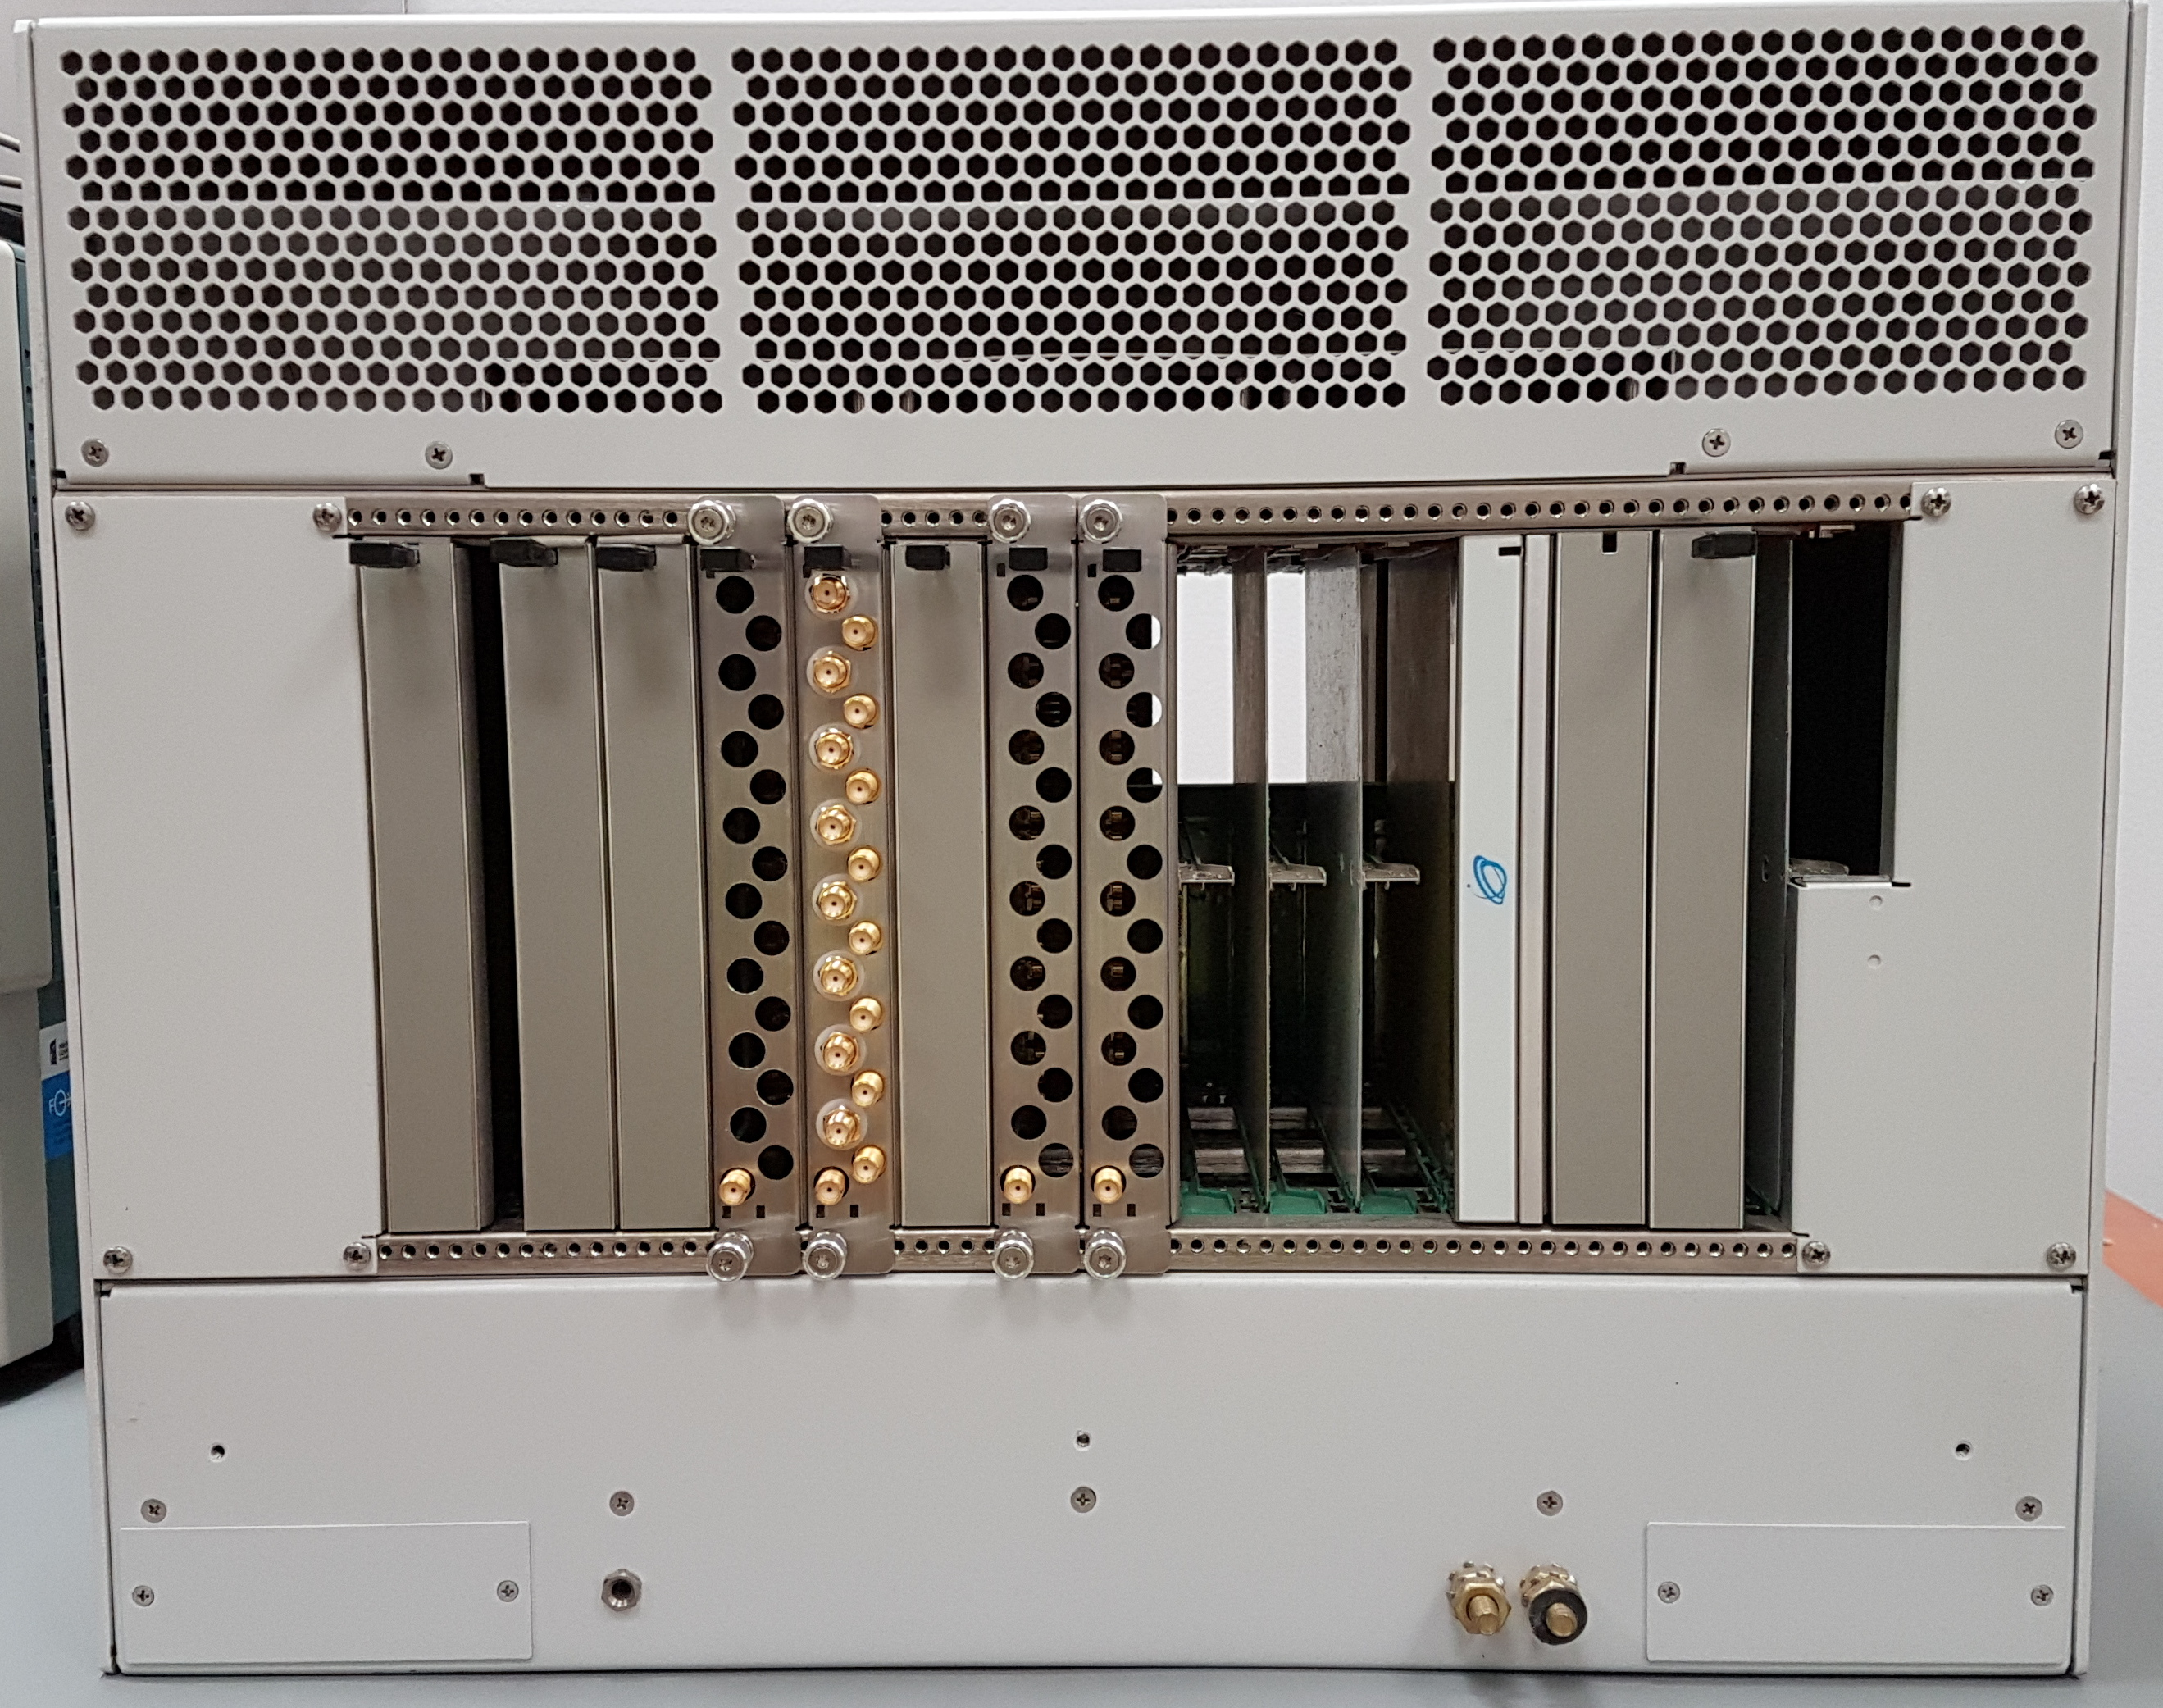
\includegraphics[width=15cm]{img/MTCA_Back.jpg}
\caption{Micro TCA chassis with 4 RTM modules inserted. One of them has
4 BaseMod AFE mezzanines installed.}
\end{figure}

\section{uTCA.4 RF Backplane}\label{utca.4-rf-backplane}

\href{http://mtca.desy.de/sites/site_mtca/content/e172206/e205636/e212584/e248086/uRFB_concept_Datasheet_19.12.2014_eng.pdf}{RF
BP datasheet}
\href{http://ieeexplore.ieee.org/stamp/stamp.jsp?arnumber=7097413\&tag=1}{RF
BP measurements}

\section{uTCA in Sinara}\label{utca-in-sinara}

\href{Metlino}{\emph{Metlino}} has been developed as an MCH optimised
for use in Sinara. It can either be the ARTIQ master or a slave,
connected to the master via DRTIO.

uTCA hardware interfaces with the extension modules either directly,
using a \href{VHDCICarrier}{VHDCI carrier}, or indirectly, using a Kasli
DRTIO slave.

To do: * Some images to illustrate what uTCA systems look like * Explain
how Baikal etc fit in * Add BP schematics that show what the
connectivity is * Any more useful information?

\section{uTCA parts and suppliers}\label{utca-parts-and-suppliers}

Add parts and suppliers from the issues list\ldots{}

\section{Schematic / Layout Viewer}\label{schematic-layout-viewer}

Mentor has a free tool called
\href{https://www.mentor.com/pcb/downloads/visecad-viewer/}{visECAD
Viewer}.
